\chapter{The VServer Control Daemon}


\section{Abstract}

In order to ease management of Virtual Private Servers a central instance is
needed to provide an open and well-known \emph{Application Programming
Interface (API)}.  The \emph{VServer Control Daemon (VCD)} is a daemon running
in the host context providing the aforementioned API via \emph{XMLRPC}, a
simple protocol for \emph{Remote Procedure Calls (RPC)} using the XML Markup
Language.


\section{Rationale}

The current user-space implementation of the Linux-VServer kernel API suffers a
mechanism to call any of the management commands regardless of the language or
location of the caller. Such callers include non-C lanuages like Python, PHP or
Ruby, remote GUIs for KDE, Gnome or even Windows as well as web control panels
for service providers.

Therefore the VServer Control Daemon defines an API accessible by any caller
capable of both the HTTP and the XMLRPC protocol -- two open standards
implemented in most common languages.


\section{Architecture}

The VServer Control Daemon consists of five major parts: the configuration
database (\emph{VXDB}), the \emph{XMLRPC Server}, the \emph{XMLRPC Clients},
the \emph{Template Management} as well as a light-weight \emph{Statistics
Collector}.

\begin{figure}[H]
	\center
	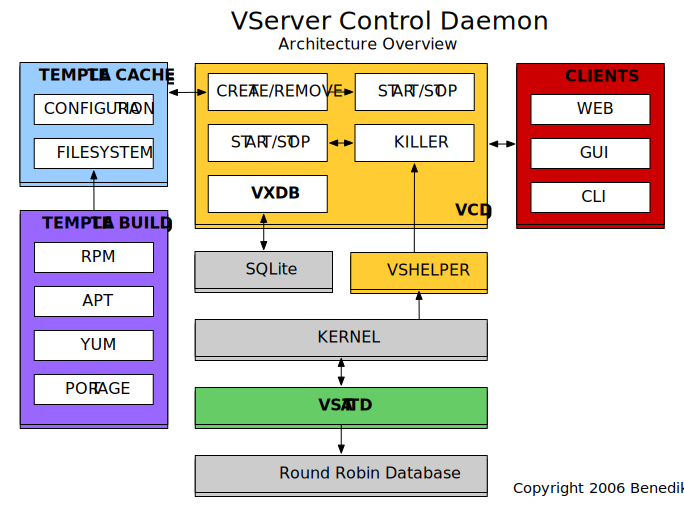
\includegraphics[scale=0.4]{intro/vcd}
	\caption{VServer Control Daemon Architecture Overview}
\end{figure}



\subsection{Configuration Database - VXDB}

The configuration database (\emph{VXDB}) stores all virtual private server
related configuration data like disk limits, CPU scheduler, or network
adresses. Furthermore the daemon stores information about its users and their
permissions as well as owned virtual servers in the database. For convenience
and size reasons the database is implemented using \emph{SQLite}.

SQLite is a small C library that implements a self-contained, embeddable,
zero-configuration SQL database engine. The decision for using SQLite as
database backend is based on the following key-features of SQLite:

\begin{itemize}
	\item Transactions are atomic, consistent, isolated, and durable even
		after system crashes and power failures
	\item Zero-configuration - no setup or administration needed
	\item A complete database is stored in a single disk file
	\item Database files can be freely shared between machines with different
		byte orders
	\item Small code footprint: less than 250KB
	\item Faster than popular client/server database engines for most common
		operations
	\item Simple, easy to use API
	\item Self-contained: no external dependencies
\end{itemize}

\subsection{The XMLRPC Server}

The \emph{XMLRPC Server} is the core of the VServer Control Daemon and
implements the XMLRPC standard for Remote Procedure Calls (RPC). XMLRPC is a
specification and a set of implementations that allow software running on
disparate operating systems, running in different environments to make
procedure calls over the Wide Area Network (Internet) or Local Area Network
(Intranet).


\subsubsection{The XMLRPC Protocol}

XMLRPC is a wire protocol that describes an XML serialization format that
clients and servers use to pass remote procedure calls to each other. There are
two features that make this protocol worth knowing. The first is that the
details of parsing the XML are hidden from the user. The second is that clients
and servers don't need to be written in the same language.

XMLRPC is designed to be as simple as possible, while allowing complex data
structures to be transmitted, processed and returned.

\begin{figure}[H]
	\center
	\includegraphics[scale=0.5]{intro/xmlrpc}
	\caption{XMLRPC data flow}
\end{figure}


Here are some examples of remote procedure call (RPC) style communications:

\begin{itemize}
	\item There is a server that can measure atmospheric temperature. A client
		anywhere in the world can ask the server at any time what the
		temperature is. The ``what temperature is it?'' request and the
		``the temperature is...'' response constitute an RPC transaction.
	\item There is a server that can turn a light on or off. A client can tell
		the server to turn the light on. A request to turn the light on and
		the acknowledgement that the light has been turned on constitute an
		RPC transaction.
	\item There is a server that knows the phone numbers of a million people.
		A client can supply a name and get back the phone number of the named
		person.
\end{itemize}

Here are some kinds of communication that are not RPC:

\begin{itemize}
	\item A long-lived connection such as an SSH login session.
	\item A high volume transfer such as an FTP download.
	\item A one-way transmission such as a UDP packet.
	\item A dialogue such as an SMTP (mail) transaction.
\end{itemize}

Based on XML nearly any application can be enabled to call methods defined by
the XMLRPC Server. The fact that XML is written in plain-text and also easily
readable by humans allows tracing and debugging with no additional overhead or
learning curve.

The server defines a global registry of methods accessible by its clients.
These methods are devided in several logical parts and seperated by a dot in
their method name. For a list of available methods see below.


\subsubsection{Authentication}

Authentication in the VServer Control Daemon is based on the cryptographic hash
function \emph{WHIRLPOOL}. WHIRLPOOL is a cryptographic hash function designed
by Vincent Rijmen and Paulo S. L. M. Barreto. The hash has been recommended by
the NESSIE project.  It has also been adopted by the International Organization
for Standardization (ISO) and the International Electrotechnical Commission
(IEC) as part of the joint ISO/IEC 10118-3 international standard.

WHIRLPOOL is a hash designed after the Square block cipher. WHIRLPOOL is a
Miyaguchi-Preneel construction based on a substantially modified Advanced
Encryption Standard (AES).  Given a message less than 2256 bits in length, it
returns a 512-bit message digest.

For security reasons the clear-text password is never stored in VXDB. The
client will send the password as plain-text - the server then creates a
WHIRLPOOL hash using the submitted password and compares its result with the
hash stored in VXDB.


\subsubsection{Access Restrictions}

For a fine-grained access control the server implements its own set of
capabilities.  A capability is a lot like the keys on your key ring. As an
example, consider your car key. It works on a specific car (it designates a
particular object), and anyone holding the key can perform certain actions
(locking or unlocking the car, starting the car, opening the glove
compartment). You can hand your car key to me, after which I can open, lock, or
start the car, but only on your car. Holding your car key won't let me test
drive my neighbor's Lamborghini.


\subsubsection{Owner Checks}

To ensure the distinction between your car and the Lamborghini another access
control system has to be implemented. Therefore the server also implements
owner checks for most of its methods. This results in an extension to the
capability model explained above. Instead of using one key per car, you can now
drive multiple cars using just one key.

Still, this model has a noticable flaw: Imagine your company has two hundred
cars and your top management should have access to all cars. Adding all members
of the management to the owner list of every single car can become a pain in
the ass very quickly. Therefore the user database in VXDB implements the
adminstrator flag. Using this flag all owner checks are passed without even
consulting the owner lists in VXDB.


\subsection{XMLRPC Clients}

The \emph{XMLRPC Clients} on the other hand connect to the XMLRPC Server using
the HTTP protocol. They need to pass authentication information, the method
name they wish to call and optionally parameters specific to the called method.
It is important to know that the connection between server and client is not
persistent, i.e. you send one request, get one answer, and the connection will
be closed afterwards. This also implies the necesity of passing authentication
information with every method call. After the request has been received and
processed the method returns a fault notification in case of any error or a
method specific return value.


\subsection{The Template Management}

The \emph{Template Management} consists of various scripts and XMLRPC methods
used to build and create new virtual private servers. The \emph{Template Build}
process assembles a complete root filesystem usable in virtual private servers,
and stores its content in a single tarball, the \emph{Template Cache.}


\subsection{The Statistics Collector}

The \emph{Statistics Collector} is a very light-weight daemon used to collect
time-series data of running virtual private servers. This data includes memory
usage, number of processes or cpu usage. The collected data is stored in
\emph{Round Robin Databases (RRD)} - the industry standard data for logging and
graphing applications - for later use in reports or graphing processes.

